\documentclass[12pt,oneside,a4paper,notitlepage]{report}

\usepackage[backend=biber,sorting=none,maxbibnames=99]{biblatex}
\usepackage{setspace}
\usepackage{graphicx}
\usepackage{syntax}
%\usepackage{wasysym}
\usepackage{textcomp}
\usepackage{newfloat}
\usepackage{enumitem}

\title{
	Implementing an Object Model for TDL\textsuperscript{TP} Expressions
}
\author{Tanel Prikk}

\DeclareFloatingEnvironment[
fileext   = logr,
listname  = {List of Grammars},
name      = Grammar,
placement = htp
]{GrammarWrapper}
\setlength{\grammarindent}{5em}
\setlength{\grammarparsep}{5pt plus 1pt minus 1pt}

\newcommand{\texttilde}{\raisebox{0.5ex}{\texttildelow}}

\addbibresource{Sources.bib}
\pagenumbering{gobble}
\singlespacing


\begin{document}
	\maketitle

	\section*{Background}
	\par Our ANTLR-generated parser is capable of building parse trees for TDL\textsuperscript{TP} expressions. The object structure of said trees is, however, dependent on the ANTLR library. Higher-level components that will work with TDL parse trees should be decoupled from this implementation detail. To achieve this, we define an independent object model which provides facilities for storage and traversal of TDL parse trees. In the future, we will also write a adapter logic for converting ANTLR TDL parse trees to objects from our independent object model.

	\newpage

	\section*{Requirements Analysis}
	\par Considering that we need to work with a parse tree (concrete syntax tree, henceforth expression tree), a suitable data structure for storing this is a rooted ordered tree. A classical implementation of such a tree is pointer-based. We provide a class diagram below:

	\begin{figure}[h]
		\begin{center}
		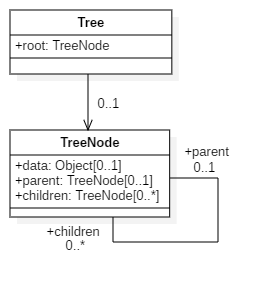
\includegraphics{Models/BasicTree}
		\end{center}
		\caption{Tree class diagram.}
		\label{fig:basic-tree}
	\end{figure}

	\par A simple approach would directly utilize the tree data structure from figure~\ref{fig:basic-tree} and provide implementations for each possible expression node that may occur in an abstract expression tree. 
	However, this is too inconvenient for clients to work with. A better approach is to take the basic \texttt{Tree} data structure as a basis for a specialized expression tree. We can encode structural rules in the APIs of the objects in an expression tree.

	\newpage

	\par To begin specifying our expression tree object model, we should take into consideration the grammar for the language, reproduced below:

	\begin{GrammarWrapper}
		\begin{grammar}
			% https://tex.stackexchange.com/questions/24886/which-package-can-be-used-to-write-bnf-grammars
			% http://texdoc.net/texmf-dist/doc/latex/mdwtools/syntax.pdf
			<Expression>	::=	'(' <Expression> ')'
			\alt 				'A' '(' <TrapsetExpression> ')'
			\alt 				'E' '(' <TrapsetExpression> ')'
			\alt 				<UnaryOp> <Expression>
			\alt 				<Expression> <BinaryOp> <Expression>
			\alt 				<Expression> '\texttilde' '\textgreater' <Expression> 
			\alt 				<Expression> '\texttilde' '\textgreater' '[' <RelOp> <NUM> ']' <Expression> 
			\alt 				'\#' <Expression> '[' <RelOp> <NUM> ']'
			
			<TrapsetExpression>	::=	'(' <TrapsetExpression> ')'
			\alt						'!' <ID>
			\alt 						<ID> '\textbackslash' <ID>
			\alt						<ID> ';' <ID>
			
			<UnaryOp>	::= '\texttilde'
			
			<BinaryOp>	::= '\&' | '|' | '-' '\textgreater' | '\textless' '-' '\textgreater'
			
			<RelOp> 	::= '\textless' | '=' | '\textgreater' | '\textless' '=' | '\textgreater' '='
			
			<ID> 		::= 'TR' <NUM>
			
			<NUM> 		::= ('0' ... '9')+
		\end{grammar}
		\caption{TDL\textsuperscript{TP} grammar}\label{bnf:modified}
	\end{GrammarWrapper}

	\newpage

	\par We can note the following simplifying factors based on grammar~\ref{bnf:modified}:
	\begin{enumerate}[label=\textbf{\arabic*.},ref=\textit{\arabic*.}]
		\item \label{simp-1} instead of treating operators as terminals, we can use them to create operator node objects in our data model;
		\item \label{simp-2} the negation operation is applicable for all logical operations - we can treat negation as an attribute for logical operation nodes (which provides a justification for having a grouping of such nodes);
		\item \label{simp-3} bound nodes (which, when treated as a whole, are a kind of terminal in TDL expression trees) are only applicable for certain logical operations; we can assume that it will not be necessary to visit such nodes separately - we can move them into logical operator node types;
		\item \label{simp-4} items \ref{simp-1} and \ref{simp-3} allow us to have the trapset symbol node type as the only leaf node type;
		\item \label{simp-5} items \ref{simp-1} and \ref{simp-3} allow us to have only operator node types as internal node types;
		\item \label{simp-6} each operator node has a restricted domain of possible operators - this can be used when defining operator node types to encode expectations on operands;
		\item \label{simp-7} all internal operator node types have a minimum arity of 1 and a maximum arity of 2 - this allows us to specify useful intermediate operator parent types which help guide and prevent clients from ignoring arity restrictions;
		\item \label{simp-8} the root node object is always an operator node.
	\end{enumerate}



	\section*{Implementation}
	\par Stub.

	\subsection*{Technology}
	\par Stub.

	\subsection*{Technical Details}
	\par Stub.

	\printbibliography[
		title=Sources
	]

\end{document}
